\documentclass[conference]{IEEEtran}
\IEEEoverridecommandlockouts
% The preceding line is only needed to identify funding in the first footnote. If that is unneeded, please comment it out.
\usepackage{cite}
\usepackage{amsmath,amssymb,amsfonts}
\usepackage{algorithmic}
\usepackage{graphicx}
\usepackage{textcomp}
\usepackage{xcolor}
\usepackage{listings}
\usepackage[ruled,vlined]{algorithm2e}
\usepackage{graphicx}
\usepackage{float}

% our changes
\usepackage[ruled]{algorithm2e}
\usepackage{amssymb}
\let\oldemptyset\emptyset
\let\emptyset\varnothing
\usepackage[T1]{fontenc}
\usepackage[utf8]{inputenc}
\usepackage{lmodern}
\usepackage{amssymb}

\def\BibTeX{{\rm B\kern-.05em{\sc i\kern-.025em b}\kern-.08em
    T\kern-.1667em\lower.7ex\hbox{E}\kern-.125emX}}
\begin{document}

\title{Video Annotation
% {\footnotesize \textsuperscript{*}Note: Sub-titles are not captured in Xplore and
% should not be used}
% \thanks{Identify applicable funding agency here. If none, delete this.}
}
\makeatletter
\newcommand{\linebreakand}{%
  \end{@IEEEauthorhalign}
  \hfill\mbox{}\par
  \mbox{}\hfill\begin{@IEEEauthorhalign}
}
\makeatother

\author{\IEEEauthorblockN{Shaashwat Jain}
\IEEEauthorblockA{\textit{dept. Computer Science and Engineering} \\
\textit{PES University}\\
Bengaluru, India \\
shaashjain213@gmail.com}
\and
\IEEEauthorblockN{Raghav Aggarwal}
\IEEEauthorblockA{\textit{dept. Computer Science and Engineering} \\
\textit{PES University}\\
Bengaluru, India \\
raghavaggarwal03.ra@gmail.com}
\linebreakand
\IEEEauthorblockN{Prof. N S Kumar}
\IEEEauthorblockA{\textit{dept. Computer Science and Engineering} \\
\textit{PES University}\\
Bengaluru, India \\
nekumar@pes.edu}
}
\maketitle

\begin{abstract}
In a multimedia-based learning system, there is a need for segmenting and organizing educational videos into topics and subtopics. The core problem in any lecture-based video is to retrieve the relevant subclips of different subtopics present in a video with accurate starting and ending time duration. Automating the segmentation process is highly desirable because a large amount of untagged educational video data is available on the Internet which does not provide any additional information regarding the context of the video except for the main title. Our approach concentrates on automatically generating the subclips of various subtopics present in a video. The proposed method exploits the automatic speech recognition (ASR) and Optical character recognition (OCR) techniques to generate the transcript of the video and apply our own topic modelling algorithm to search for meaningful context-related subtopics in the transcript. We further extend our model to the concept of Kernel density estimator (KDE) to tackle the problem of occurrence of the same subtopic, having a significant duration, at multiple places in a video. The obtained durations of each subtopic helps in generating the subclips. Using video content with available description and title, more insights can be gained which indeed are useful for the students in structuring the content of video according to topics.
\end{abstract}

\begin{IEEEkeywords}
Topic modelling, video segmentation, OCR, speech recognition, KDE, multimedia
\end{IEEEkeywords}


\section{Introduction}

Digital Communication today is not only reliant on text but also on multimedia like images, audio, and video. Video has become a popular way to teach in computer based teaching (CBT), e-learning and communication between the users due to which there is a huge amount of video data available on the internet increasing storage space and bandwidth. Many researchers have shown that multimedia instruction can enhance students’ problem-solving and understanding skills [1]. The content of most lecture videos contains more than one topic or subtopic. In order to facilitate student learning and minimize learning time, lecture videos usually are segmented into smaller topics for browsing [2].\\ 
Professional institutes like MIT, IIT’s, NIT’s and other engineering colleges are making videos of their lectures. The main objective of NPTEL and OpenCourseWare program is to enhance the quality of engineering education by providing curriculum based video lecture series. This initiation has been carried out by MIT, several IITs and IISc Bangalore as a project [3]. Generally university lectures take hours and generate a large video file and sometimes without a transcript. Consequently, it becomes difficult for learners to access the lecture content efficiently as it is not at one’s ease to stare at a computer screen for a long lecture, especially when they are only interested in some parts of the lecture rather than the whole. The educational videos content which is available on YouTube, University websites usually provide the information about the main topic by means of title and description. There is no additional information regarding:-
\begin{itemize}
	\item What are name of the subtopics present in the video?
	\item What is the duration of these subtopics?
	\item Where do all these subtopics occur?
\end{itemize}

These questions made us think that is it possible to retrieve the subclips of the subtopic from the video containing all its occurrences and how to determine when a subtopic has ended. Manually segmenting the video is the best way to find the subtopics but this approach is very time/money consuming and considering the amount of video lecture data available on the internet, it is very tough to achieve the goal. Therefore, the objective of this paper is to develop effective and efficient automated approaches to find subclips of different topics present in lecture videos. All these facts drive us to automate the task of generating the subclips of lecture video. We divided the task of obtaining them in three
parts:-

\paragraph{Generating transcript}
In the first part, the goal is to generate the transcript of the video if it is not available. With the help of Google speech-recognition and by analysing the sound decibels in the lecture video it will generate a transcript with all the sentence breaks and pauses in order to map each sentence in transcript with the timing of audio. This mapping also helps us to keep track of time.

\paragraph{Analysing transcript}
In the second part, the goal is to find the meaningful subtopics in the transcript and retrieve the duration of each subtopic even if it has multiple occurrences. In order to achieve this we have used our own Topic Modelling \textbf{targeted n-gram algorithm}. This algorithm provides us a list of possible topics/subtopics accounting frequency of each word along with other factors such as surrounding grammar.\\
\indent To double check the possible subtopics OCR data is used from video as most educational videos use a powerpoint presentation to teach and it also provides a list of possible subtopics.

\paragraph{Extracting segments}
In the third part, the goal is obtain the subclips of all the meaningful subtopics. Using the generated list of subtopics and their occurrence timings the duration of these subtopics are calculated using the concept of box and whisker plot. Finally we merge all of the subclips to get a single topic video.

\textbf{The main contributions of this research work are summarized as follows:-}
\begin{enumerate}
\item A unique, yet updated approach to a more targeted n-gramming technique using POS (parts of speech) tagging for finding meaningful sections from a particular sentence.
\item Analysing and processing redundancies and further estimating meaning in the observable section i.e. potential concept using a frequency based approach on the audio as well as visual.
\item Assigning ranked importance to each potential concept for a time mapped subclipping approach on sections of the entire video where the concept is predominant, further merging these sections into one whole concept or topic.
\end{enumerate}

\subsection*{\textbf{Motivation}}
Because of COVID-19, the schools and Universities are compelled to switch over to an online mode of teaching. Therefore, a large amount of multimedia data i.e video, audio, and images is getting generated every day and most of it is unprocessed data which is available on the internet. Most of the already existing educational videos are insufficient to provide comprehensive details about the content present in the video with the help of title. Such video data fall under the category of our testing data. An aspirant learner may have to go through the complete video to gain the knowledge of all the subtopics which are present in the video. Moreover, if he is searching for a particular subtopic then he has to go through the entire video or a set of videos to find the starting point of a particular subtopic or might not even find that subtopic. Considering all these scenarios this whole procedure is like a treasure hunt which is very cumbersome and time-consuming. So, the need of the hour is to automate this process of finding subtopics and their first occurrence along with their durations in order to save time. To solve this problem we have built a model that provides the user with sub clippings of all the relevant subtopics that are possible in the video.\\
\\
The rest of the paper is organized as follows: Section 2 illustrates the detailed methodology for our proposed solution while Section 3 and Section 4 are Results and conclusion respectively.


\begin{figure*}[h]
    \centering
    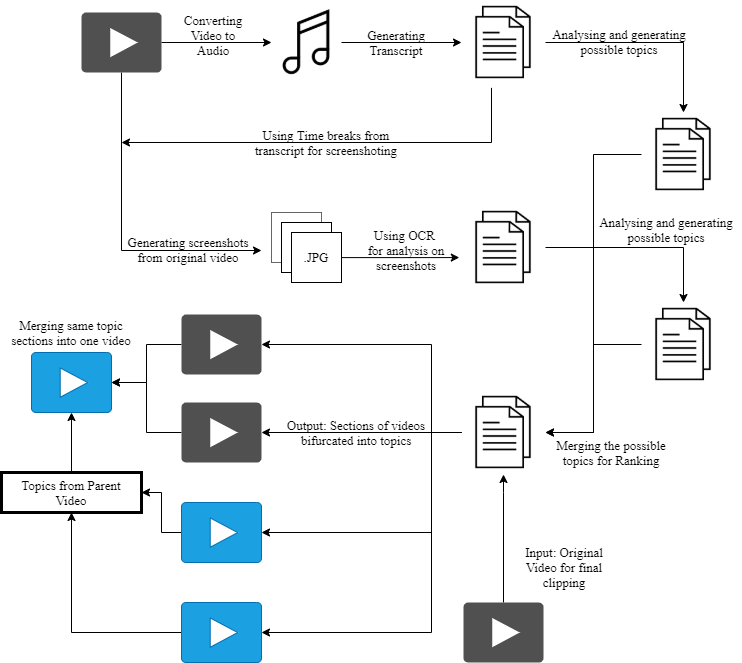
\includegraphics[width=\textwidth]{image2.png}
    \caption{Diagram of proposed solution framework}
    \label{fig:inputs_loss_mask}
\end{figure*}

\section{Methodology}
\subsection{Transcript Generation}
\subsubsection{Audio}
The first step in this elaborated process is by converting our video to audio and work upon it. For the model, the most important part is the transcript of the audio. While generating one we can take two approaches:-
\begin{itemize}
\item Constant time approach
\item Variable time approach
\end{itemize}

The constant time approach is a tedious approach and doing analysis on stop words through the technique is quite painful and also produces inaccurate results. We choose the much easier but space consuming approach of variable time. For this approach, using silences on stop words is the trick. We tweak our subclips based on the amount of gap a person gives between sentences ( by analysing decibels) and further split them to further generate text from them. There are various Speech-to-text engines available online which use hidden Markov models and various other models to generate accurate text. This prediction while being accurate still induces some amount of error in the transcript. There are many more methods to get a transcript. Many sources provide a manually written transcript with their videos for better understanding. We tend to use either of the two approaches mentioned to generate a grammatically well suited transcription for our analysis.\\

\subsubsection{Visual}
Extending our analysis to not only using audio information, we use video information which can provide extended analysis in the case some visual aid is being used to explain some concept. We have used the concept \textit{"capture and identify"} to find meaningful data from the video. Illustrating this further, take the video and capture the screen from it after a certain threshold for each video which can be decided by our audio transcript. Further, use OCR techniques (eg: tesseract-OCR) on the captured image file and document our data in similar fashion as that of the audio transcript. OCR can be erroneous so we take care of that by using the NLTK dictionary on the words other than nouns present in the data and subsequently remove the words not found. Finally, for doing so we needed to treat redundancy in our data for which we used a pattern matching algorithm.\\
\indent The basic algorithm for pattern matching predates, and is a little fancier than, an algorithm published in the late 1980’s by Ratcliff and Obershelp under the hyperbolic name \textit{“gestalt pattern matching”} [4]. We further compare subsequent results and decide on a threshold for the percentage of a match. Only if the threshold isn’t crossed we use the string in our video generated transcription.

\subsection{Topic Finding}
In this section we present one of the main contributions of the paper. We will go through our transcript and do an analysis on our transcript for the most suitable results.

\subsubsection{\textbf{A targeted approach to n-grams}}
To find any meaningful topic, the first approach taken was the n-gram approach. n-grams are Markov models that estimate words from a fixed window of previous words. n-gram probabilities can be estimated by counting in a corpus and normalizing(the maximum likelihood estimate). [5] Unigram taggers are based on a simple statistical algorithm: for each token, assign the tag that is most likely for that particular token. An n-gram tagger is a generalization of a unigram tagger whose context is the current word, n, together with the part-of-speech tags of the n-1 preceding tokens. The process of classifying words into their parts of speech and labeling them accordingly is known as part-of-speech tagging, POS-tagging, or simply tagging [6].\\
\indent The problem with this approach was the amount of garbage topics. To find an alternative, we designed a 
\begin{figure}[H]
  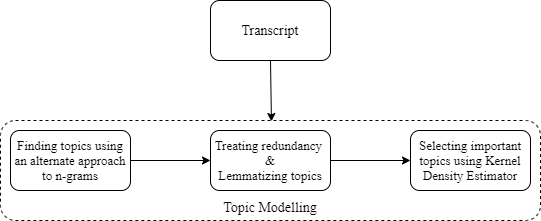
\includegraphics[width=\linewidth]{image1.png}
  \caption{Functioning of Topic Modelling}
  \label{fig:Topic Modelling}
\end{figure}

classification model taking the pretext as an inspiration. Prior to this, evaluating the transcript and filtering it to sentences based on each time stamp was crucial. Subsequently, performing POS-tagging on each sentence to get a probabilistic model of each word and it’s grammar gave a start to this approach. For our analysis we went with the spacy[4] neural model for precision tagging of words. Once we get the POS tagged corpora, we start our analysis for chunks of words on it. Algorithm 1 will give us a better understanding.

\begin{algorithm}
\SetAlgoLined
\DontPrintSemicolon
\SetKwInOut{Input}{input}
\SetKwInOut{Output}{output}
\Input{A set of references to the pos tagged sentences, S, which contains references to their respective POS tags with property, pos. “NN” is the tagged nouns and “JJ” is the tagged adjectives.}
\Output{A set of references to all output topics, O}
	$S = \emptyset$\\
	\For{$s \in S$}{
		\If{$s.pos \in "NN"$}{
			$n = 1$\\
			$topic = s$
			}
			\While{$(s+n) \in "NN"$}{
				$topic += s+n$\\
			}
			$O = O \cup topic$\\
		\If{$s.pos \in "JJ"$}{
			$n = 1$\\
			$topic = s$\\
			\While{$(s+n) \in "NN"$}{
				$topic += s+n$\\
				$n += 1$\\
				}
			\If{$n $>$ 1$}{
				$O = O \cup topic$\\
				}
		}
	}

\caption{Noun and adjective based Targeted n-grams approach}
\end{algorithm}


We find these chunks by using the corpora’s tagged “NN” - nouns and “JJ” - adjectives. The algorithm dictates that in the transcript when we find nouns, we go on to find continued words which are nouns so we can get a good idea about the topics. Further, for a better output, extending our analysis to chunks of adjectives followed by nouns seemed like the right approach. For the adjectives to have meaning it is an essential for the chunk to end with a noun. As the chunks are found, distinguish between the ones which have one word and which have multiple words. The one word chunks can be specified as just occurrences of nouns while the ones with multiple words can be inferred to as possible topics for the video.\\
\indent This usage of the model got us very accurate topics for our sample videos and compared to traditional n-gram techniques we got about 50-60\% less garbage values on an average. Further, it would help for the list of all topics to be converted into a dictionary of topics where the keys could be the count of occurrences of the topic in our transcript.

\subsubsection{\textbf{Treating Redundancy}}
Once we have a dictionary of topics, there is a need to treat the topics which have very close meaning. To do so, first, treat the language of the topics. For that use a technique called lemmatization. [8] The standard WordNet lemmatizer has a restricted dictionary. For more accurate results you can resort to open source lemmatizers. For our approach we have resorted to a more manual approach of treating some source lemmas. Once the topics are treated, remove the topics which were redundant by adding their occurrences to one key.\\
\indent Now, to treat similar topics which our lemmatizer couldn't detect, use the previously talked about technique for pattern matching. The algorithm gives us a \textit{"ratio of match"} for two topics, which may then be compared using the O($n^2$) method. Simply, compare every topic with all others to get a \textit{"ratio of match"} for all of them. Once this is computed, decide a threshold for filtering the topics which are above the threshold and merge the topics to form a cleaner dictionary of topics and occurrences.\\
\indent Using these methods we get an accurate dictionary with correctly represented occurrences which gravely helps further our analysis.

\subsubsection{\textbf{Filtering topics using Kernel Density Estimator}} 

Now, lets dive in deeper into the classification of the topics. Having found all the filtered topics, the next step is to classify and remove the insignificant ones which have very little or no meaning throughout the video. For explaining purposes, If we have some topic which was mentioned casually in the video, it won’t need to be identified as a talked about topic in the video. For doing so, we already have a data structure representing every topic and how many times it has occurred in the whole speech. The need now, is a threshold for selecting out of the many topics, which of them have significant importance. Many techniques can be used to do so. For an initial approach, a fairly simple model of finding the Interquartile Range (IQR) value of our data and then finding a threshold using the 75th percentile data point and adding $1.5*IQR$ gives a very good idea of the problem at hand. The results which we got were quite promising but certain improvements were required.\\
\indent KDE is an extended analysis of smoothening the histogram to plot a smooth, symmetric curve. A classical approach of density estimation is the histogram. The KDE is one of the most famous methods for density estimation. Here is the formal definition of the KDE. The KDE is a function

$$ \hat{p}_{n}(x) = \frac{1}{nh}\sum\limits_{i=1}^n K(\frac{X_{i}-x}{h})$$

\indent where K(x) is called the kernel function that is generally a smooth, symmetric function such as a gaussian and h > 0 is called the smoothing bandwidth that controls the amount of smoothing. Basically, the KDE smoothes each data point $X_{i}$ into small density bumps and then sums all these small bumps together to obtain the final density estimate. [6] The K(x) function can be chosen among many popular density functions. In theory, the kernel function does not play a key role. But sometimes in practice,they do show some difference in the density estimator.[6] The smoothing bandwidth plays an important role in the density estimation. The lower we get a bandwidth the rougher our curve is. For this analysis, staying in between the under-smoothing and over-smoothing range of the parameter is best.\\
\indent	The Gaussian Kernel of the KDE gives the results needed. The Gaussian Kernel function K(x) is defined as:
$$K(x) = \frac{1}{\sqrt{2\pi}}e^\frac{-x^2}{2}$$

\indent Further, using the curve to our benefit, extract its maximas and minimas, and averaging the first off values to get an initial threshold and eliminating the petty topics which were auto-generated, majorly the ones which had under the threshold occurrences in a fairly large video. Once we get our topics we can rank them which we will see thoroughly in the next section.\\
\\
This process is done for both our transcripts which give us accurate topics from the OCR data and our speech. The OCR data is more significant for verification of speech data as the amount of error is quite significant. The dictionary of single worded topics from OCR data makes a quite significant contribution to our further analysis.

\subsection{Ranking}
In this section we will conclude our topic finding analysis by summing all our raw topics and their occurrences into a finished dictionary of the most significant ones. Here we also introduce another significant method for finding significant topics, the keyword derived topics.
	Keyword Derived Topics are useful in the case of analysis of multiple videos by some particular content creator or professor who teaches in a particular field of interest. For explanation purposes, if the field of interest is \textit{'A'} and all the videos are based on that field of interest then whenever a topic is encountered which is related, similar or exactly \textit{'A'} then our algorithm will give that topic a preference in ranking until some other topic overpowers it by some significant margin.\\
\indent For completing our analysis on the two dictionaries generated respectively by our speech and video transcripts, first try to find the topics in the speech transcript and match each word in the topic with the generated OCR dictionary. For a n-word topic, n > 0, firstly try to find a match for each i word, 1 $\leq$ i $\leq$ n, and store the occurrences of the OCR transcript and find the minimum of all occurrences. Then try to find if the exact topic was found in the OCR transcript. If an exact match is found, add the occurrence count to the dictionary. If in case an exact match isn’t found, add the previously computed minimum value to the dictionary. This way we get a more accurate representation about the topics and their significance in the analysis. This is followed by adding a threshold value for the Keyword Derived Topics in the dictionary which gives us a final dictionary on which, apply the KDE analysis from the previous subsection and filter the topics which hold less significance.\\
\indent Indexing the whole video onto a single roof topic is finding the topic which has either:
\begin{itemize}
\item Occurred the most number of times
\item Ranges for the most time in the video
\item Contains some keyword which overpowers it
\end{itemize}
\indent Therefore, we get multiple topics from which the user can pick the significance and assign the topic. Finally, there is a need to timestamp the acquired topics in a manner that the topics are chosen between intervals when they are most significant and not just span most of the video. The last section will describe how we implement that.


\subsection{Subclipping}
After getting the list of all the possible subtopics, the transcript and the subtopics are converted to lowercase. This is done to prevent the miss match of the character while searching for the subtopics in the transcript. As we encounter a subtopic in transcript, it’s timing is appended in a list and repeating this procedure for all the subtopics, a dictionary is obtained where subtopic name is the key and the list of timing of occurrence for each subtopic in the video is the value. This comprises the < key, value > pair.\\
\indent Now to determine when a subtopic is starting and ending, we make a new list which contains the difference of consecutive time values which are present in the dictionary. If the difference value is greater than a particular threshold then we mark that point and get the subclip from the beginning till that marked point. This gives a single clip of a subtopic. This particular threshold is calculated by using the box plot. Using the list of difference values, a box plot is made and all the values which are greater than the upper whisker of the box plot is the threshold value which tells the ending point of each clip. Then merging these clips gives a subclip of one subtopic. Repeating this process for all subtopics gives the subclip of all subtopics in a video.


\section{Results}

\section{Conclusion and Future perspective}
\begin{thebibliography}{9}
\bibitem{1} 
W. Zhang, Chapter 8, “Multimedia Technology, Education and Learning”, Technological Innovations in Literacy and Social Studies Education [online], 1995. Available: http://tiger.core.missouri.edu 
\bibitem{2} 
M. R. Halvorsen, “Content-based lecture video indexing,” Master’s thesis ,2007.
\bibitem{3} 
NPTEL (National Programme on Technology Enhanced Learning), http://nptel.iitm.ac.in
\bibitem{4}
https://docs.python.org/3/library/difflib.html
\bibitem{5}
https://web.stanford.edu/~jurafsky/slp3/3.pdf
\bibitem{6}
https://www.nltk.org/book1ed/ch05.html
\bibitem{7}
https://spacy.io/models
\bibitem{8}
https://www.nltk.org/book/ch03.html
\bibitem{9}
http://faculty.washington.edu/yenchic/17Sp403/Lec7-density.pdf
\bibitem{10} 
Covington, P.; Adams, J.; Sargin, E. Deep neural networks for youtube recommendations. In Proceedings of the 10th ACM Conference on Recommender Systems, New York, NY, USA, 7 September 2016; pp. 191–198.
\end{thebibliography}

\end{document}



